\documentclass[11pt]{article}
\usepackage[margin=1in]{geometry}
\usepackage{amsmath,amssymb,amsthm}
\usepackage{enumitem}
\usepackage{tikz}

\newtheorem{theorem}{Theorem}
\newtheorem{lemma}{Lemma}
\newtheorem{proposition}{Proposition}

\newcommand{\R}{\mathbb{R}}
\DeclareMathOperator{\Area}{Area}
\DeclareMathOperator{\diam}{diam}

\title{The smallest ellipse containing two unit disks has area
$\tfrac{3\sqrt3}{2}\,\pi$\\[2pt]
\large (a hand-checkable proof)}
\author{}
\date{}

\begin{document}
\maketitle

\begin{theorem}
Among all ellipses containing two closed unit disks with disjoint interiors, the minimum
area is
\[
A \;=\; \frac{3\sqrt3}{2}\,\pi \;\approx\; 8.1621,
\]
attained by the axis-aligned ellipse with semi-axes
\[
a=\frac{3\sqrt2}{2}=\frac{3}{\sqrt2}\ \text{(major)},\qquad
b=\frac{\sqrt6}{2}=\sqrt{\tfrac32}\ \text{(minor)},
\]
with the two disks centered at $(\pm1,0)$ on the major axis, touching each other at
the origin. Each disk is internally tangent to the ellipse at two points,
$\bigl(\pm\tfrac32,\pm\tfrac{\sqrt3}{2}\bigr)$.
\end{theorem}

\noindent (We say two disks are \emph{interior-disjoint} if their interiors do not meet; for unit
disks this is equivalent to their centers being at distance $\ge2$.) The proof has four steps:
\begin{itemize}[leftmargin=1.6em,itemsep=1pt]
  \item \textbf{Step 1} (normalization): the ellipse may be taken axis-aligned and centered at the
        origin.
  \item \textbf{Step 2} (the main reduction): any ellipse holding two interior-disjoint unit disks
        also holds the single disk centered at $(1,0)$ on the major axis.
  \item \textbf{Step 3} (lower bound): one boundary point of that disk, together with the AM--GM
        inequality, forces the area to be $\ge\tfrac{3\sqrt3}{2}\pi$, with equality only at
        $a^2=\tfrac92,\ b^2=\tfrac32$.
  \item \textbf{Step 4} (upper bound): that ellipse does contain two interior-disjoint unit disks,
        by a one-line perfect-square check.
\end{itemize}

%======================================================================
\section*{Step 1. Normalization}

Let $E$ be any ellipse containing two interior-disjoint unit disks $D_1,D_2$ with centers
$p_1,p_2$. An ellipse is an affine image of a disk; in particular it has a center $O_E$
(its center of symmetry) and two perpendicular axes of symmetry, the major and minor axes.

Apply the rigid motion (a rotation about $O_E$ followed by a translation) that sends $O_E$
to the origin and the major axis to the $x$-axis. Rigid motions preserve areas, the radii
of the two disks, and their disjointness, and carry $E$ to an axis-aligned, origin-centered
ellipse
\begin{equation}
E:\quad \frac{x^2}{a^2}+\frac{y^2}{b^2}\le 1,\qquad a\ge b>0, \tag{$\star$}
\end{equation}
where $a$ is the semi-major and $b$ the semi-minor axis, and $\Area(E)=\pi ab$. (If $E$ is a
circle, $a=b$; the argument below specializes harmlessly, and we shall see it is not
optimal.) Thus \emph{without loss of generality every competitor has the form $(\star)$},
and we must
\[
\textbf{minimize } \pi ab \quad\text{subject to: $E$ contains two interior-disjoint unit disks.}
\]
Throughout, write
\[
u:=a^2,\qquad v:=b^2,\qquad u\ge v>0 .
\]

%======================================================================
\section*{Step 2. Reduction to the symmetric touching configuration}

We prove that for a fixed ellipse $(\star)$, two interior-disjoint unit disks fit inside $E$ if and
only if the single unit disk centered at $(1,0)$ fits. The forward direction is the substance of this
step; the converse is immediate. Consequently ``$E$ holds two disjoint unit disks'' reduces to the
one-disk condition analyzed in Step~3, and the extremal configuration is the symmetric pair touching
at the origin with centers on the major axis.

\subsection*{2a. The set of admissible centers is convex and doubly symmetric}

Let
\[
  C:=\{\,z\in\R^2:\ z+B(0,1)\subseteq E\,\}
\]
be the set of centers of unit disks contained in $E$ (the inner parallel body of $E$).

\emph{$C$ is convex.} Let $z_1,z_2\in C$ and $0\le\lambda\le1$. For every $|w|\le1$ we have
$z_1+w\in E$ and $z_2+w\in E$, so by convexity of $E$,
\[
  \bigl(\lambda z_1+(1-\lambda)z_2\bigr)+w
   =\lambda(z_1+w)+(1-\lambda)(z_2+w)\in E .
\]
As this holds for all such $w$, $\lambda z_1+(1-\lambda)z_2\in C$.

\emph{$C$ is symmetric about both coordinate axes.} The reflections $(x,y)\mapsto(-x,y)$ and
$(x,y)\mapsto(x,-y)$ map $E$ to itself, and carry the unit disk at $z$ to the unit disk at the
reflected center; so they preserve $C$. ($C$ is nonempty iff $b\ge1$, i.e.\ $v\ge1$, the obvious
requirement that one unit disk fit.)

\subsection*{2b. Feasibility forces a \emph{unit vector} into $C$}

Two unit disks are interior-disjoint iff their centers are at distance $\ge2$. So suppose
$p,q\in C$ with $|p-q|\ge2$. By the triangle inequality $|p|+|q|\ge|p-q|\ge2$, so at least one
center --- say $p$ --- satisfies $|p|\ge1$. Since $O\in C$ (because $b\ge1$) and $p\in C$, convexity
gives the segment $[O,p]\subset C$; as $|p|\ge1$, its point at distance $1$ from $O$,
\[
m':=\frac{p}{|p|}\quad(\text{a \emph{unit vector}, }|m'|=1),
\]
lies in $C$. Thus: \emph{if $E$ holds two disjoint unit disks, then $C$ contains a
unit vector $m'$}, i.e.\ some unit disk with center on the unit circle fits in $E$.

\subsection*{2c. The major-axis center is the easiest unit vector to contain}

Intuitively, $E$ is widest along its major ($x$-)axis, so a unit disk has the most room to fit when
its center is pushed out along that axis; the major-axis center $(1,0)$ should be the easiest unit
vector to contain. We make this precise. For a center $P$, write $D_P=\{P+w:|w|\le1\}$ for the unit
disk centered there. Since $E=\{Q\le1\}$ with $Q(x,y)=x^2/u+y^2/v$,
\[
  D_P\subseteq E\quad\iff\quad N(P):=\max_{Y\in D_P}Q(Y)\ \le\ 1 .
\]

\begin{lemma}\label{lem:major}
If $u\ge v$, then $N\bigl((1,0)\bigr)\le N(m')$ for every unit vector $m'$. Consequently, if the
unit disk centered at some unit vector $m'$ lies in $E$, so does the unit disk centered at $(1,0)$.
\end{lemma}

The proof rests on one elementary property of $Q$.

\paragraph{Radial monotonicity.} In polar form $X=r(\cos\psi,\sin\psi)$,
\begin{equation}\label{eq:radial}
  Q(X)=r^2\Bigl(\tfrac{\cos^2\psi}{u}+\tfrac{\sin^2\psi}{v}\Bigr)
       =r^2\Bigl(\tfrac1v-\bigl(\tfrac1v-\tfrac1u\bigr)\cos^2\psi\Bigr).
\end{equation}
Since $u\ge v$, the coefficient $\tfrac1v-\tfrac1u\ge0$, so \emph{at a fixed distance $r$ from $O$,
$Q(X)$ decreases as $\cos^2\psi$ grows}: $Q$ is smallest along the $x$-axis and increases as $X$ turns
toward the $y$-axis. Thus two points equidistant from $O$ satisfy $Q(X')\ge Q(X)$ whenever
$\cos^2\psi'\le\cos^2\psi$ --- i.e.\ whenever $X'$ makes the larger angle with the $x$-axis.

\begin{proof}[Proof of Lemma~\ref{lem:major}]
Reflecting in the coordinate axes maps $E$ to itself and a fitting disk to a fitting disk, and leaves
$N$ unchanged; so we may assume $m'=(\cos\varphi,\sin\varphi)$ with $\varphi\in[0,\tfrac\pi2]$. Let $R$
be the rotation by $\varphi$ about $O$. The unit ball is rotation-invariant, so $R$ carries the disk at
$(1,0)$ onto the disk at $m'=R(1,0)$:
\[
  D_{m'}=R\,D_{(1,0)} .
\]

Let $B_0\in D_{(1,0)}$ attain $N\bigl((1,0)\bigr)=\max_{Y\in D_{(1,0)}}Q(Y)$, and write
$B_0=(1+c,\,s)$ with $c^2+s^2\le1$. Replacing the offset $(c,s)$ by $(|c|,|s|)$ gives the point
$(1+|c|,\,|s|)$, which is still in $D_{(1,0)}$ (the offset has the same length) and has $Q$ at least as
large: $(1+|c|)^2\ge(1+c)^2$ and $|s|^2=s^2$, so each term of $Q$ is $\ge$ the original. Hence a
maximizer with $c,s\ge0$ exists, and we take $B_0=(1+c,s)$ with $c,s\ge0$. Its polar angle $\psi_0$
then satisfies
\[
  \tan\psi_0=\frac{s}{1+c}\le1\qquad(\text{since }s\le1\le1+c),
\]
so $\psi_0\in[0,\tfrac\pi4]$.

Now $R\,B_0\in R\,D_{(1,0)}=D_{m'}$, so $N(m')\ge Q(R\,B_0)$. The point $R\,B_0$ is at the same distance
from $O$ as $B_0$, with polar angle $\psi_0+\varphi$. Since $\psi_0\le\tfrac\pi4$ and $\varphi\le\tfrac\pi2$,
\[
  \psi_0\ \le\ \psi_0+\varphi\ \le\ \psi_0+\tfrac\pi2\ \le\ \pi-\psi_0 ,
\]
so $\psi_0+\varphi$ lies in the band $[\psi_0,\pi-\psi_0]$, on which $\cos^2$ never exceeds
$\cos^2\psi_0$. By radial monotonicity~\eqref{eq:radial}, $Q(R\,B_0)\ge Q(B_0)$. Therefore
\[
  N(m')\ \ge\ Q(R\,B_0)\ \ge\ Q(B_0)\ =\ N\bigl((1,0)\bigr),
\]
and in particular $N(m')\le1$ forces $N\bigl((1,0)\bigr)\le1$.
\end{proof}

\subsection*{2d. Conclusion of the reduction}

Combining 2b and 2c: if $E$ holds two disjoint unit disks, then $C$ contains a unit vector
$m'$, and by the Lemma the disk at $(1,0)$ then lies in $E$. Conversely, if the disk at
$(1,0)$ lies in $E$ then by the $x\mapsto-x$ symmetry so does the disk at $(-1,0)$, and these
two unit disks are interior-disjoint (centers distance $2$ apart). Therefore:
\begin{quote}
\itshape
For the fixed ellipse $(\star)$, $E$ holds two interior-disjoint unit disks
$\iff$ the unit disk centered at $(1,0)$ lies in $E$.
\end{quote}
The right-hand condition no longer mentions the disk positions. Thus, for bounding the area, we may
replace ``$E$ holds two disjoint unit disks'' by the single condition that the disk centered at
$(1,0)$ lies in $E$; Steps 3 and 4 analyze exactly this condition.

%======================================================================
\section*{Step 3. The lower bound, from one boundary point and AM--GM}

Let $E$ be any ellipse containing two interior-disjoint unit disks. By Step~1 we may assume the
normalized form $(\star)$, $E=\{x^2/u+y^2/v\le1\}$ with $u=a^2\ge v=b^2$, and by Step~2 the unit disk
centered at $(1,0)$ lies in $E$. We need only \emph{one} point of that disk. The boundary point
\[
  \Bigl(\tfrac32,\ \tfrac{\sqrt3}{2}\Bigr)=(1,0)+\Bigl(\tfrac12,\tfrac{\sqrt3}{2}\Bigr),
  \qquad\text{at distance }1\text{ from }(1,0),
\]
lies in $E$, so
\[
  \frac{(3/2)^2}{u}+\frac{(\sqrt3/2)^2}{v}\le1,
  \qquad\text{i.e.}\qquad \frac{9}{u}+\frac{3}{v}\le4 .
\]
Set $X=\dfrac9u$ and $Y=\dfrac3v$, so $X,Y>0$ and $X+Y\le4$. By the AM--GM inequality,
\[
  XY\ \le\ \Bigl(\frac{X+Y}{2}\Bigr)^2\ \le\ 4 .
\]
But $XY=\dfrac{27}{uv}$, so $\dfrac{27}{uv}\le4$, i.e.\ $uv\ge\dfrac{27}{4}$, and therefore
\[
  \Area(E)=\pi ab=\pi\sqrt{uv}\ \ge\ \pi\sqrt{\tfrac{27}{4}}=\frac{3\sqrt3}{2}\,\pi .
\]
Equality forces $X=Y$ and $X+Y=4$, i.e.\ $X=Y=2$: then $\dfrac9u=2$ and $\dfrac3v=2$, giving
$u=\tfrac92$ and $v=\tfrac32$. This is the only ellipse that can attain the bound.

%======================================================================
\section*{Step 4. The construction attains it}

It remains to exhibit a valid configuration of area $\tfrac{3\sqrt3}{2}\pi$. Take $u=a^2=\tfrac92$,
$v=b^2=\tfrac32$ and the disks centered at $(\pm1,0)$ (so $ab=\sqrt{27/4}=\tfrac{3\sqrt3}{2}$, and the
two disks are at distance $2$, with disjoint interiors). By the $x\mapsto-x$ symmetry of $E$ it
suffices to check the disk at $(1,0)$: a boundary point is $(1+c,\,s)$ with $c=\cos t$, $s=\sin t$,
and there
\[
  Q=\frac{(1+c)^2}{u}+\frac{1-c^2}{v}
   =\frac{(1+c)^2}{9/2}+\frac{1-c^2}{3/2}
   =-\tfrac49c^2+\tfrac49c+\tfrac89=:g(c).
\]
Multiplying $1-g(c)$ by $uv=\tfrac{27}{4}>0$ gives the perfect square
\[
  \tfrac{27}{4}\bigl(1-g(c)\bigr)=3c^2-3c+\tfrac34=3\Bigl(c-\tfrac12\Bigr)^2\ \ge0,
\]
so $g(c)\le1$ for all $c\in[-1,1]$: the disk at $(1,0)$, and by symmetry the disk at $(-1,0)$, lies
in $E$. Equality holds exactly at $c=\tfrac12$ (i.e.\ $t=\pm\tfrac\pi3$), the four tangency points
$\bigl(\pm\tfrac32,\pm\tfrac{\sqrt3}{2}\bigr)$; the two disks touch at the origin. Thus this ellipse
genuinely contains two interior-disjoint unit disks and has area $\tfrac{3\sqrt3}{2}\pi$.

Combining Steps 3 and 4: the minimum area is exactly $\tfrac{3\sqrt3}{2}\pi$, and the minimizing
ellipse is $\tfrac{x^2}{9/2}+\tfrac{y^2}{3/2}\le1$, unique up to rigid motion. $\blacksquare$

%======================================================================
\section*{Figures}

\begin{center}
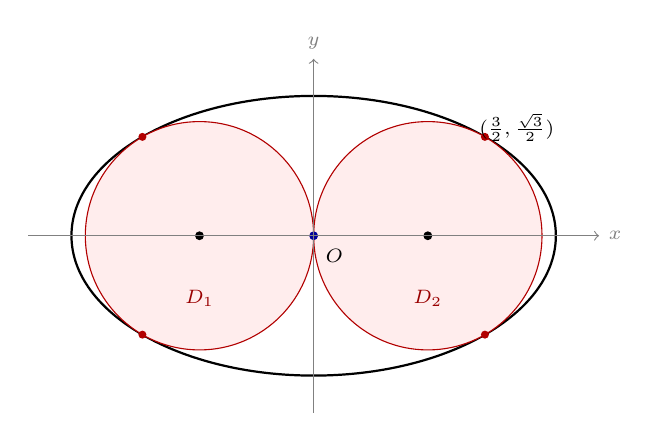
\begin{tikzpicture}[scale=1.45]
  % ellipse a=3/sqrt2 ~ 2.1213, b=sqrt(1.5) ~ 1.2247
  \pgfmathsetmacro{\aa}{2.12132034}
  \pgfmathsetmacro{\bb}{1.22474487}
  \draw[thick] (0,0) ellipse ({\aa} and {\bb});
  % unit disks at (+-1,0)
  \draw[red!70!black,fill=red!7] (1,0) circle (1);
  \draw[red!70!black,fill=red!7] (-1,0) circle (1);
  % centers and touch point
  \fill (1,0) circle (1.1pt); \fill (-1,0) circle (1.1pt);
  \fill[blue!60!black] (0,0) circle (1.1pt);
  \node[below right] at (0.02,-0.03) {\scriptsize $O$};
  % tangency points (3/2, +- sqrt3/2) and (-3/2, +-sqrt3/2)
  \pgfmathsetmacro{\ty}{0.8660254}
  \foreach \sx in {1,-1}{\foreach \sy in {1,-1}{
     \fill[red!70!black] (\sx*1.5,\sy*\ty) circle (1.0pt);
  }}
  % axes
  \draw[->,gray] (-2.5,0)--(2.5,0) node[right]{\scriptsize $x$};
  \draw[->,gray] (0,-1.55)--(0,1.55) node[above]{\scriptsize $y$};
  \node at (1,-0.0) {};
  \node[red!60!black] at (1.0,-0.55) {\scriptsize $D_2$};
  \node[red!60!black] at (-1.0,-0.55) {\scriptsize $D_1$};
  \node at (1.78,0.95) {\scriptsize $(\tfrac32,\tfrac{\sqrt3}{2})$};
\end{tikzpicture}
\end{center}

\noindent The optimal ellipse $x^2/\tfrac92+y^2/\tfrac32=1$ with the two unit disks
centered at $(\pm1,0)$, touching at $O$. Each disk is internally tangent to the ellipse at
two points $\bigl(\pm\tfrac32,\pm\tfrac{\sqrt3}{2}\bigr)$ (red dots).

%======================================================================
\section*{Remarks}

\emph{Uniqueness of the ellipse.} The equality analysis in Step~3 pins the optimal ellipse exactly:
AM--GM equality and the boundary constraint together force $u=\tfrac92$, $v=\tfrac32$. So the
minimizing ellipse $\tfrac{x^2}{9/2}+\tfrac{y^2}{3/2}\le1$ is unique up to rigid motion.

\emph{Where the difficulty lies.} Once Step~2 is in hand, the bound is short: the single forced point
$(\tfrac32,\tfrac{\sqrt3}{2})$ and one application of AM--GM give it, with no optimization. The only
genuinely geometric content is Step~2 --- that for an ellipse with horizontal major axis, if two
disjoint unit disks fit at all, then the disk centered at $(1,0)$ fits. Naive global estimates do not
suffice for the constant: the two disks have combined area $2\pi\approx6.28$, well below
$\tfrac{3\sqrt3}{2}\pi\approx8.16$, so the bound cannot come from an area comparison alone.

\medskip
\footnotesize\noindent The two algebraic facts used above --- the boundary-point inequality with
AM--GM, and the tangency certificate $\tfrac{27}{4}(1-g)=\tfrac34(2c-1)^2$ --- have also been verified
by exact symbolic computation, and the entire argument has been formalized and machine-checked in
Lean~4 with mathlib; an independent numerical optimization over the full problem (free ellipse and
free centers) returns the stated optimum
$a^2=\tfrac92,\ b^2=\tfrac32$ with the disks at $(\pm1,0)$.

\end{document}
